\documentclass[11pt]{article}
\usepackage[margin=1in]{geometry}
\usepackage{amsmath,amssymb,amsfonts}
\usepackage{booktabs}
\usepackage{xcolor}
\usepackage{hyperref}
\usepackage{cleveref}
\usepackage{graphicx}
\usepackage{enumitem}
\graphicspath{{figures/screening_resolution/}}
\hypersetup{colorlinks=true,linkcolor=blue!60!black,citecolor=blue!60!black,urlcolor=blue!60!black}

\title{\textbf{Supplementary Information}\\CrossPiezo: Elite-Tail Instability in Cross-Database Piezoelectric Screening}
\author{Anonymous Author(s)}
\date{3 August 2026}
\begin{document}
\maketitle

\tableofcontents
\newpage

\section{Supplementary notes}

\subsection{Portfolio estimand definition (Note~1)}

The portfolio benchmark reports two related quantities.
\emph{Worst-source recall} is a material-level (micro) metric: it counts how many of the top-$q^* n$ materials selected by a strategy are also present in the JARVIS and MP elite sets, divided by $q^* n$, with no group weighting.
\emph{Paired difference in recall} is the difference between the material-level worst-source recall of the strategy and that of the better single-source baseline, computed on the full observed panel.

The confidence interval reported in Table~S3 uses a \emph{full-procedure grouped bootstrap}.
Each replicate:
(i) resamples reduced-formula groups with replacement and assigns distinct bootstrap identities to duplicated occurrences;
(ii) recomputes source-specific rankings and top-$q^*$ elite sets on the bootstrap sample;
(iii) re-runs the portfolio strategy and both single-source baselines;
(iv) computes the improvement over the better single source within that replicate.
The reported 95\% interval is the percentile bootstrap interval of these replicate differences.
The point estimate is fixed on the full-panel selections and is exactly the arithmetic difference of the Recall column; the bootstrap captures uncertainty from group resampling and re-selection.

The ``better single source'' is determined per replicate for the interval; the main-text point estimate uses the full-panel better source (here JARVIS-only and MP-only are tied on P0 F1 at $q^*=10\%$, $b=1.0$).
The portfolio analysis is presented as a risk-management illustration, not as a validated method comparison or as evidence of physical truth.

\subsection{Structure matching and manual audit (Note~2)}

The CrossPiezo-Invariant-v1 panel was constructed from relaxed CIFs shared by the Materials Project (MP) and JARVIS.
The matching pipeline is: (i) load all processed MP and JARVIS piezoelectric records; (ii) compute structure-level overlaps by compositional reduced formula and relaxed-lattice similarity; (iii) apply a frozen similarity threshold to obtain candidate pairs; (iv) perform a response-blind manual audit of the top-matched candidates using a frozen rule set.
The audit was response-blind: the auditor did not see piezoelectric response values when deciding whether a candidate pair represented the same or a distinct structure.
All audit decisions, exclusion reasons and ambiguous cases are recorded in the frozen panel-membership file.

The frozen matcher tolerances are: fractional length tolerance $\ell_\mathrm{tol}=0.2$, site tolerance $s_\mathrm{tol}=0.3$\,\AA, angle tolerance $5^\circ$, primitive-cell reduction enabled, and lattice scaling enabled (see ``configs/matching.yaml'').
P0 ($n=573$) is the full set of accepted structure matches; P2 ($n=207$) is the subset passing tighter RMS-distance and lattice-distance thresholds ($\mathrm{RMS}_\mathrm{thr}\approx0.0078$\,\AA, lattice-distance threshold $\approx0.0036$).
Table~\ref{tab:si_matching_audit} gives the resulting distance distributions.
Figure~\ref{fig:si_distance_discrepancy} shows that relaxed-structure distance is only weakly associated with cross-source F1 rank discrepancy (Spearman $\rho\approx-0.09$), so large response disagreement is not simply an artefact of loose structure matching.

\subsection{Tensor invariants and conventions (Note~3)}

All piezoelectric response values are piezoelectric stress tensors $\mathbf{e}$ in C/m$^2$ with full Cartesian $3\times3\times3$ components.
The three coordinate-invariant scalars are:
\begin{itemize}[noitemsep]
\item F1, Cartesian Frobenius norm $\|\mathbf{e}\|_F$;
\item F3, true collinear longitudinal maximum $\max_{\|\mathbf{n}\|=1} |n_i e_{ijk} n_j n_k|$ computed by numerical optimisation over the unit sphere;
\item F4, Kelvin/Mandel operator norm on symmetric strain, computed from the Mandel representation of the $6\times3$ piezoelectric tensor.
\end{itemize}
Voigt-to-Cartesian conversion follows the standard convention $11\to xx$, $22\to yy$, $33\to zz$, $23\to yz$, $13\to xz$, $12\to xy$ with factor-of-two handling for shear components as appropriate for the stress tensor.
No sign conventions, unit conversions or coordinate rotations were applied silently; all transformations are recorded in the repository transformation history.

\subsection{Bootstrap, quantile and tie handling (Note~4)}

Screening-resolution curves are evaluated at quantiles $q=1\%,2\%,\dots,50\%$.
The chance-adjusted Jaccard overlap is $\widetilde J_q = (J_q - \mathbb{E}[J_q])/(1 - \mathbb{E}[J_q])$, where $\mathbb{E}[J_q]$ is the exact hypergeometric expectation under independent rankings.
Simultaneous 95\% confidence bands for the screening-resolution curve use a paired bootstrap with a studentized sup-norm critical value; this bootstrap resamples matched material pairs (rows) because the curve itself is a cross-sectional function of the ranked universe and the band is constructed for fixed quantiles.

For property-control comparisons and the portfolio benchmark, bootstrap resampling is by reduced-formula group to respect the dependence among entries sharing a composition.
In the portfolio full-procedure bootstrap, duplicated groups create distinct bootstrap identities so that re-selection and elite-set sizes are computed on the expanded bootstrap sample.
The random seed, number of replicates, studentization details, tie handling and $k$ rounding are recorded in the Phase~7C configuration and result files.
Ties in source rankings are broken by stable sorting; duplicate reduced formulae are retained in the ranking but noted in the panel metadata.
The persistent-onset criterion requires the lower confidence bound to exceed a threshold $\delta$ for at least five consecutive quantiles.

\subsection{Source workflow and tensor conventions (Note~5)}

Both JARVIS and MP report the piezoelectric stress tensor $\mathbf{e}$ in C/m$^2$ using the same Voigt order ($xx,yy,zz,yz,xz,xy$) and the same engineering-shear factor-of-two convention.
JARVIS values are expressed in the source-structure Cartesian frame; MP values are expressed in the MP IEEE-oriented structure frame.
Before any response comparison, MP structures are aligned to JARVIS structures (or vice versa) with a frozen ``pymatgen'' ``StructureMatcher'' configuration and the recovered rotation is applied to the MP Cartesian tensor.
The three reported scalars (F1, F3, F4) are coordinate-frame invariants, so they are unaffected by the source-specific structure-frame choice.

Several calculation settings are not documented in the release metadata used by CrossPiezo: exchange--correlation functional, pseudopotential family, DFPT vs finite-difference ionic response, plane-wave cutoff, k-point density, relaxation thresholds, primitive vs conventional defaults, and sign-convention history.
These items are therefore reported as unknown rather than assumed identical (see \path{docs/mp_vs_jarvis_conventions.md}).
The repository convention audit (\path{scripts/run_convention_audit.py}) confirms that F1, F3 and F4 are rotation invariant, that Voigt/Cartesian conversion and engineering-shear handling are internally consistent, and that the F3 optimiser converges to a dense-grid brute-force oracle.
This audit rules out low-level convention errors in the CrossPiezo pipeline; it does not prove that JARVIS and MP use identical calculation settings.

\subsection{Screening resolution vs conventional ranking diagnostics (Note~6)}

Screening resolution is reported through the chance-adjusted Jaccard curve $\widetilde J_q$ and its area (nAUCC) because these metrics focus on the elite tail where cross-database disagreement is largest.
For comparison, Table~\ref{tab:si_baseline_metrics} and Figures~\ref{fig:si_synthetic_baseline}--\ref{fig:si_baseline_comparison} report conventional diagnostics:
plain Jaccard $J_q$, chance-adjusted Jaccard $\widetilde J_q$, overlap coefficient, precision/recall at $k$, Rank-Biased Overlap (RBO) with $p=0.95$, top-weighted Kendall $\tau$ on the union of the two top-$k$ sets, and top-weighted Spearman $\rho$ on the same union.

These diagnostics illustrate that two rankings can have high global correlation yet disagree on the top few percent of candidates.
The synthetic example in Figure~\ref{fig:si_synthetic_baseline} constructs two length-100 rankings with global Kendall $\tau \approx 0.98$ but disjoint top-$5\%$ sets; global metrics are near-perfect while top-$5\%$ precision and Jaccard are zero.
On P0 F1 the same pattern holds: global Kendall $\tau$ is high (see Table~\ref{tab:si_baseline_metrics}), but elite-tail agreement is near chance for small $q$.

\section{Supplementary figures}

\begin{figure}[htbp]
\centering
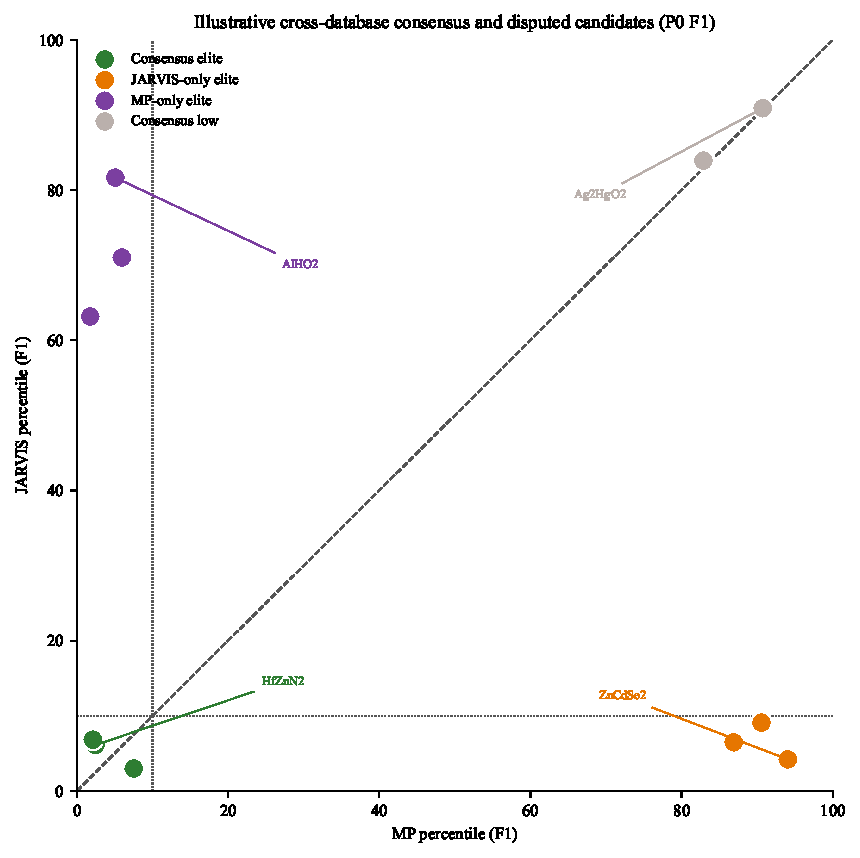
\includegraphics[width=0.95\textwidth]{fig4_illustrative_candidates}
\caption{Illustrative cross-database consensus and disputed candidates on P0 F1.
Points show JARVIS versus MP percentiles for consensus elite (green), JARVIS-only elite (orange), MP-only elite (purple) and consensus low (grey) materials.
The dashed diagonal marks equal ranking; dotted lines mark the 10\% elite threshold.
These examples are illustrative and are not adjudicated as physically correct or incorrect.}
\label{fig:si_candidates}
\end{figure}

\begin{figure}[htbp]
\centering
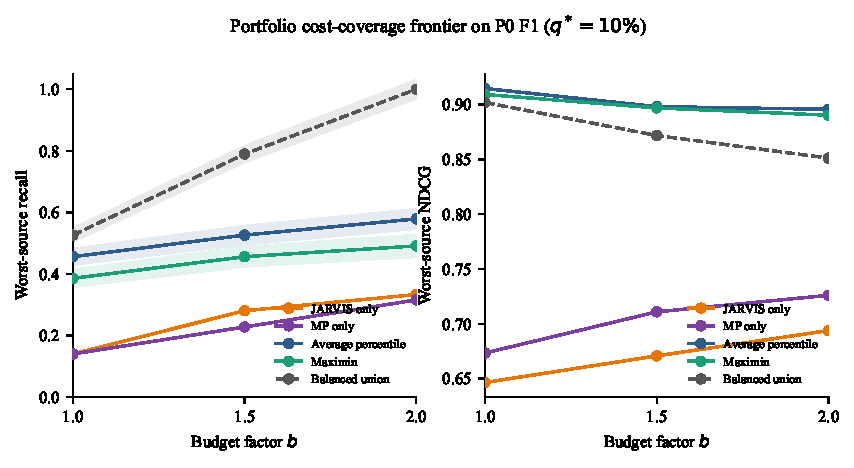
\includegraphics[width=0.95\textwidth]{fig5_portfolio_frontier}
\caption{Portfolio cost--coverage frontier on P0 F1 ($q^*=10\%$).
Worst-source recall (left) and NDCG (right) are plotted against budget factor $b$ for the best single-source baselines and three source-robust aggregation strategies.
The vertical dashed line marks the equal-budget analysis at $b=1.0$.
Aggregation changes the coverage--quality trade-off but does not validate physical truth.
See Note~1 for the distinction between material-level recall and group-mean paired differences.}
\label{fig:si_portfolio}
\end{figure}

\begin{figure}[htbp]
\centering
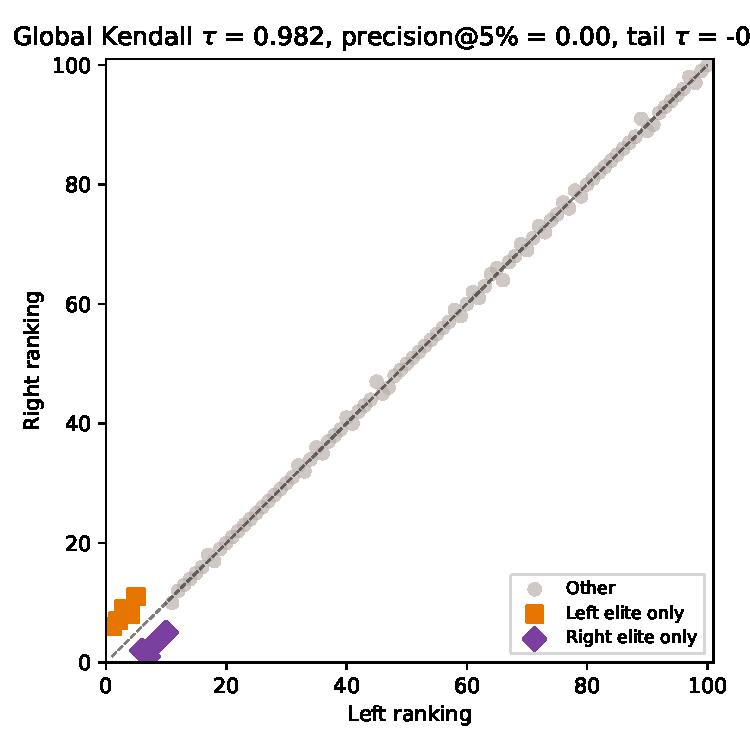
\includegraphics[width=0.95\textwidth]{fig_synthetic_baseline_metrics}
\caption{Synthetic motivating example for screening resolution.
Two length-100 rankings are constructed with global Kendall $\tau \approx 0.98$ but disjoint top-$5\%$ sets, showing that high global rank correlation does not guarantee agreement on elite-screening decisions.
The reported conventional metrics (global $\tau$, Spearman $\rho$, Rank-Biased Overlap) are near-perfect while top-$5\%$ precision and Jaccard are zero.
See Note~6 for the full metric definitions.}
\label{fig:si_synthetic_baseline}
\end{figure}

\begin{figure}[htbp]
\centering
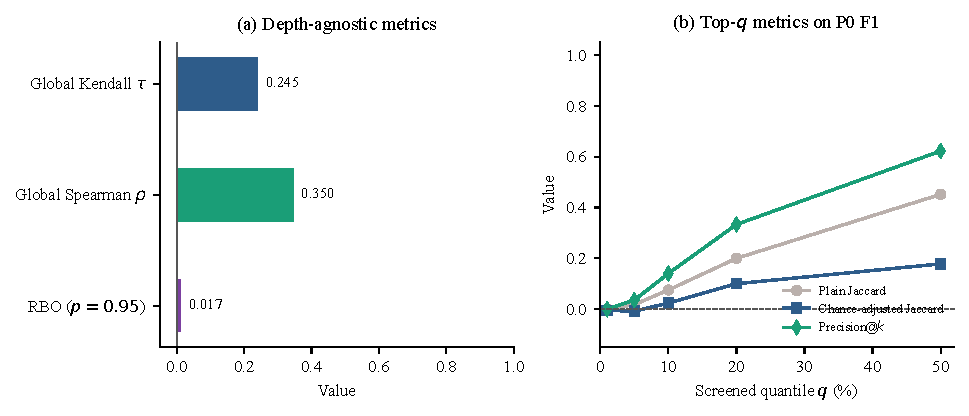
\includegraphics[width=0.95\textwidth]{fig_s1_baseline_metric_comparison}
\caption{Comparison of conventional ranking diagnostics and screening-resolution on P0 F1.
Top panels report global and top-$q$ Kendall $\tau$ and Spearman $\rho$; bottom panels report chance-adjusted Jaccard $\widetilde J_q$, plain Jaccard $J_q$, precision@$k$, and Rank-Biased Overlap.
Global correlation is high, but elite-tail agreement is near-chance for small $q$.
See Table~\ref{tab:si_baseline_metrics} for the numerical values and Note~6 for definitions.}
\label{fig:si_baseline_comparison}
\end{figure}

\begin{figure}[htbp]
\centering
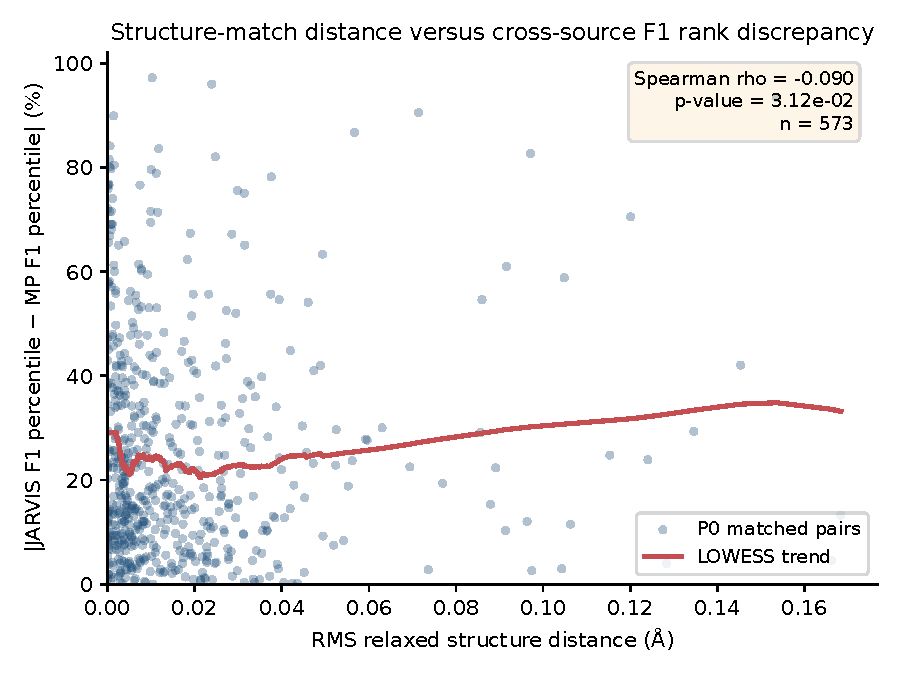
\includegraphics[width=0.95\textwidth]{fig_s2_distance_vs_rank_discrepancy}
\caption{Relaxed-structure RMS distance versus absolute F1 percentile gap for the 573 P0 matched pairs.
The weak Spearman correlation ($\rho\approx-0.09$) indicates that large cross-database response disagreement is not dominated by poorly matched structures.
The LOWESS curve is illustrative and is not a fitted model.}
\label{fig:si_distance_discrepancy}
\end{figure}

\section{Supplementary tables}

\begin{table}[htbp]
\small
\setlength{\tabcolsep}{4pt}
\centering
\caption{Corrected high-response sensitivity for P0 F1 at $f=0.10$ and $f=0.25$.}
\label{tab:si_highresponse}
\begin{tabular}{lcccccc}
\toprule
Method \& $f$ \& $N$ \& $	au$ \& CI \& nAUCC \& CI \\
\midrule
Dual-high & 10\% & 58 & 0.035 & [-0.193, 0.239] & -0.046 & [-0.118, 0.044] \\
JARVIS anchor & 10\% & 57 & 0.209 & [-0.062, 0.374] & 0.053 & [-0.061, 0.191] \\
MP anchor & 10\% & 57 & -0.053 & [-0.235, 0.137] & -0.018 & [-0.104, 0.090] \\
Pooled (exploratory) & 10\% & 58 & -- & [--, --] & -0.155 & [--, --] \\
Dual-high & 25\% & 143 & 0.070 & [-0.046, 0.181] & 0.031 & [-0.034, 0.102] \\
JARVIS anchor & 25\% & 143 & -0.019 & [-0.141, 0.105] & -0.006 & [-0.070, 0.070] \\
MP anchor & 25\% & 143 & 0.039 & [-0.083, 0.154] & 0.007 & [-0.052, 0.078] \\
Pooled (exploratory) & 25\% & 144 & -- & [--, --] & -0.100 & [--, --] \\
\bottomrule
\end{tabular}
\end{table}


\begin{table}[htbp]
\small
\setlength{\tabcolsep}{4pt}
\centering
\caption{Property-control comparison on P0. The same-field copy flag is raised when more than 5\% of finite matched pairs have identical JARVIS/MP values.}
\label{tab:si_controls}
\begin{tabular}{lcccccccc}
\toprule
Attribute \& $N$ \& $	au$ \& 95\% CI \& nAUCC \& 95\% CI \& $\Delta\tau$ \& $\Delta$nAUCC \& Copy flag \\
\midrule
Volume \& 573 \& 0.967 \& [0.963, 0.971] \& 0.918 \& [0.901, 0.936] \& 0.722 \& 0.813 \&  \\
Band gap \& 573 \& 0.908 \& [0.890, 0.923] \& 0.897 \& [0.864, 0.908] \& 0.663 \& 0.792 \&  \\
Energy above hull \& 573 \& 0.611 \& [0.547, 0.670] \& 0.533 \& [0.455, 0.592] \& 0.366 \& 0.428 \& $\checkmark$ \\
Dielectric trace \& 573 \& 0.482 \& [0.418, 0.547] \& 0.286 \& [0.228, 0.344] \& 0.236 \& 0.181 \&  \\
\bottomrule
\end{tabular}
\end{table}


\begin{table}[htbp]
\small
\setlength{\tabcolsep}{4pt}
\centering
\caption{Equal-budget ($b=1.0$) portfolio results on P0 F1 ($q^*=10\%$).
Paired differences are versus the better single-source baseline and are computed as material-level worst-source recall differences using a full-procedure grouped bootstrap: each replicate resamples reduced-formula groups with replacement, assigns distinct identities to duplicated occurrences, re-runs the portfolio strategy and both single-source baselines, and recomputes the improvement (see Note~1).}
\label{tab:si_portfolio}
\begin{tabular}{lccccc}
\toprule
Strategy \& Recall \& NDCG \& Coverage \& $\Delta$Recall \& 95\% CI \\
\midrule
JARVIS only \& 0.140 \& 0.646 \& 0.099 \& 0.000 \& [0.000, 0.000] \\
MP only \& 0.140 \& 0.673 \& 0.099 \& 0.000 \& [0.000, 0.000] \\
Average percentile \& 0.456 \& 0.915 \& 0.099 \& 0.316 \& [0.172, 0.362] \\
Borda \& 0.456 \& 0.915 \& 0.099 \& 0.316 \& [0.172, 0.362] \\
Maximin \& 0.386 \& 0.909 \& 0.099 \& 0.246 \& [0.107, 0.286] \\
Intersection first \& 0.456 \& 0.915 \& 0.099 \& 0.316 \& [0.172, 0.362] \\
Balanced union \& 0.526 \& 0.902 \& 0.099 \& 0.386 \& [0.273, 0.441] \\
Disagreement abstention \& 0.456 \& 0.915 \& 0.099 \& 0.316 \& [0.172, 0.362] \\
Minimax oracle \& 0.474 \& 0.915 \& 0.099 \& 0.333 \& [0.250, 0.414] \\
\bottomrule
\end{tabular}
\end{table}


\begin{table}[htbp]
\small
\setlength{\tabcolsep}{4pt}
\centering
\caption{Portfolio worst-source recall on P0 F1 across budget factors $b=1.0, 1.5, 2.0$.}
\label{tab:si_budget}
\begin{tabular}{lccc}
\toprule
Strategy \& $b=1.0$ \& $b=1.5$ \& $b=2.0$ \\
\midrule
JARVIS only \& 0.140 \& 0.281 \& 0.333 \\
MP only \& 0.140 \& 0.228 \& 0.316 \\
Average percentile \& 0.456 \& 0.526 \& 0.579 \\
Maximin \& 0.386 \& 0.456 \& 0.491 \\
Balanced union \& 0.526 \& 0.789 \& 1.000 \\
\bottomrule
\end{tabular}
\end{table}


\begin{table}[htbp]
\small
\setlength{\tabcolsep}{3pt}
\centering
\caption{Baseline ranking diagnostics on P0 F1 (global Kendall $\tau$ = 0.245, global Spearman $\rho$ = 0.350).
Columns are, from left to right: screened quantile $q$, corresponding top-$k$ set size, plain Jaccard, chance-adjusted Jaccard $\widetilde J_q$, overlap coefficient, precision/recall at $k$ (equal for paired rankings), Rank-Biased Overlap with $p=0.95$, top-weighted Kendall $\tau$ on the union of the two top-$k$ sets, top-weighted Spearman $\rho$ on the same union, and the partial nAUCC of the band containing $q$ (elite $1$--$10$, intermediate $10$--$20$, broad $20$--$50$).}
\label{tab:si_baseline_metrics}
\begin{tabular}{rccccccccc}
\toprule
$q$ (\%) & $k$ & Plain $J$ & $\widetilde J_q$ & Overlap & Prec@$k$ & RBO$_{0.95}$ & $\tau_{q}$ & $\rho_{q}$ & Band nAUCC \\
\midrule
1 & 5 & 0.000 & -0.005 & 0.000 & 0.000 & 0.017 & -0.289 & -0.588 & 0.003 \\
5 & 28 & 0.018 & -0.007 & 0.036 & 0.036 & 0.017 & -0.532 & -0.760 & 0.003 \\
10 & 57 & 0.075 & 0.024 & 0.140 & 0.140 & 0.017 & -0.386 & -0.613 & 0.003 \\
20 & 114 & 0.200 & 0.100 & 0.333 & 0.333 & 0.017 & -0.331 & -0.489 & 0.076 \\
50 & 286 & 0.452 & 0.178 & 0.622 & 0.622 & 0.017 & -0.080 & -0.112 & 0.145 \\
\bottomrule
\end{tabular}
\end{table}


\begin{table}[htbp]
\small
\setlength{\tabcolsep}{3pt}
\centering
\caption{Frozen structure-matching audit summary. P0 is the full relaxed-structure matched universe; P2 is the tighter subset retained by the RMS and lattice thresholds recorded in ``panel\_counts.json''.}
\label{tab:si_matching_audit}
\resizebox{\textwidth}{!}{%
\begin{tabular}{lcccccccccccc}
\toprule
Panel & Count & Expected & RMS mean & RMS med. & RMS max & Max mean & Max med. & Max max & Lat. mean & Lat. med. & Lat. max \\
\midrule
P0 & 573 & 573 & 0.017 & 0.009 & 0.168 & 0.025 & 0.013 & 0.298 & 0.066 & 0.004 & 1.897 \\
P2 & 207 & 207 & 0.003 & 0.003 & 0.008 & 0.004 & 0.004 & 0.019 & 0.001 & 0.001 & 0.004 \\
\bottomrule
\end{tabular}%
}
\end{table}



\end{document}
